\documentclass[tikz,border=6pt]{standalone}
\usepackage{amsmath,amssymb,mathtools,physics,bm,nicefrac,wasysym}
\usepackage{xcolor}

\definecolor{colone}{RGB}{180,60,60}
\definecolor{coltwo}{RGB}{60,110,180}
\definecolor{colthree}{RGB}{60,140,80}

\definecolor{accent}{HTML}{A13D2C}
\definecolor{accent2}{HTML}{2B5F6B}
\definecolor{muted}{HTML}{5A564F}
\definecolor{panel}{HTML}{F8F6F0}
\definecolor{linecol}{HTML}{D8D2C4}
\definecolor{ink}{HTML}{1E1C1A}
\definecolor{astroblue}{HTML}{1B4F72}
\definecolor{astrodark}{HTML}{17202A}
\definecolor{sunyellow}{HTML}{E8A33D}

\usetikzlibrary{calc,arrows.meta,positioning,decorations.pathreplacing,decorations.markings,angles,quotes,shapes.geometric}
\usepackage{tikz-3dplot}

\newcommand{\vecr}{\vec r}
\newcommand{\vecL}{\vec L}
\newcommand{\vecA}{\vec A}
\newcommand{\vecf}{\vec f}
\newcommand{\vecF}{\vec F}
\newcommand{\vecp}{\vec p}
\newcommand{\avg}[1]{\left\langle #1\right\rangle}
\newcommand{\vecx}{\vec x}
\newcommand{\hatn}{\hat n}
\newcommand{\rhat}{\hat r}
\newcommand{\phihat}{\hat\phi}
\newcommand{\thetahat}{\hat\theta}
\newcommand{\note}[1]{\textcolor{blue!60!black}{\textit{[#1]}}}

\newcommand{\LST}{\mathrm{LST}}
\newcommand{\GST}{\mathrm{GST}}
\newcommand{\GMST}{\mathrm{GMST}}
\newcommand{\GAST}{\mathrm{GAST}}
\newcommand{\LMST}{\mathrm{LMST}}
\newcommand{\LAST}{\mathrm{LAST}}
\newcommand{\UT}{\mathrm{UT}}
\newcommand{\UTC}{\mathrm{UTC}}
\newcommand{\TAI}{\mathrm{TAI}}
\newcommand{\TT}{\mathrm{TT}}
\newcommand{\TDB}{\mathrm{TDB}}
\newcommand{\JD}{\mathrm{JD}}
\newcommand{\MJD}{\mathrm{MJD}}
\newcommand{\EoT}{\mathrm{EoT}}
\newcommand{\SNR}{\mathrm{SNR}}
\newcommand{\RON}{\mathrm{RON}}



\begin{document}
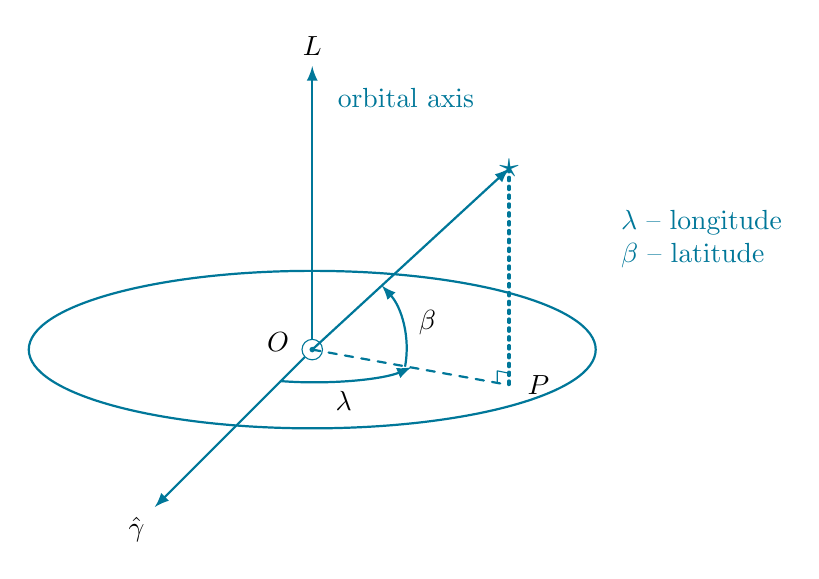
\begin{tikzpicture}[>=latex, line join=round, line cap=round]
		
		% Custom Cyan color
		\definecolor{mycyan}{RGB}{0, 119, 153}
		
		% Coordinates
		\coordinate (O) at (0, 0);
		\coordinate (L) at (0, 3.6);
		\coordinate (Gamma) at (-2.0, -2.0);
		
		% Position vector & orthogonal projection point on the xy-plane
		\coordinate (Star) at (2.5, 2.3);
		\coordinate (Proj) at (2.5, -0.45);
		
		% 1. Orbital Plane Ellipse
		\draw[mycyan, thick] (0,0) ellipse (3.6cm and 1.0cm);
		
		% 2. Vertical Axis L (Orbital Axis)
		\draw[->, mycyan, thick] (O) -- (L) node[above, black] {$L$};
		\node[mycyan, right] at (0.2, 3.2) {orbital axis};
		
		% 3. Reference Axis (\hat{\gamma})
		\draw[->, mycyan, thick] (O) -- (Gamma) node[below left, black] {$\hat{\gamma}$};
		
		% 4. Origin Label and Circle
		\node[black, left=2pt] at (-0.1, 0.1) {$O$};
		\draw[mycyan, fill=white] (O) circle (0.13cm);
		\fill[mycyan] (O) circle (0.035cm);
		
		% 5. Primary Vectors and Projection Lines
		\draw[->, mycyan, thick] (O) -- (Star);
		\draw[dashed, mycyan, thick] (O) -- (Proj) node[right=3pt, black] {$P$};
		\draw[dotted, mycyan, very thick] (Star) -- (Proj);
		
		% 6. Right-Angle Symbol at Point P
		\draw[mycyan, thin] (2.35, -0.42) -- (2.35, -0.27) -- (2.5, -0.30);
		
		% 7. Star Marker
		\node[mycyan, scale=1.4] at (Star) {$\star$};
		
		% 8. Longitude (\lambda) Arc with explicit curved 3D plane projection
		% Parametric arc: R_x = 1.5cm, R_y = 0.4167cm (aspect ratio 3.6)
		% Starts on \hat{\gamma} at (-0.400, -0.400) [t = 254.5 deg]
		% Ends on line OP at (1.260, -0.227) [t = 327.1 deg]
		\draw[mycyan, thick, ->] (-0.400, -0.400) arc[start angle=254.5, end angle=327.1, x radius=1.5cm, y radius=0.4167cm];
		\node[black] at (0.40, -0.65) {$\lambda$};
		
		% 9. Latitude (\beta) Elevation Arc from OP to OStar
		\draw[mycyan, thick, ->] (1.18, -0.21) arc[start angle=-10.2, end angle=42.6, radius=1.2cm]
		node[midway, right=2pt, black] {$\beta$};
		
		% 10. Legend
		\node[mycyan, align=left, anchor=west] at (3.8, 1.4) {
			$\lambda$ -- longitude \\
			$\beta$ -- latitude
		};
		
	\end{tikzpicture}
\end{document}
